\documentclass[]{article}
\usepackage{amsmath}
\usepackage{bm}
\usepackage{graphicx}
\usepackage[hmargin={2.54cm,2.54cm},vmargin={2.54cm,2.54cm}]{geometry}
\usepackage{subfigure}

\graphicspath{{../Images/}}

\title{Solving the Helmholtz equation using multigrid}

\begin{document}
\maketitle
The code is the same as in Tutorials/LinearSolvers/ABecLaplacian\_F except that the variables in the equation are changed. The code has two options in the inputs file --  prob\_type 1 solves a Poisson problem with Dirichlet boundary conditions, and prob\_type 2 solves a Helmholtz problem with Neumann boundary conditions. In this document, the Helmholtz problem with Neumann BCs is described. 
\section{Governing equation}
This tutorial solves the Helmholtz equation (the Poisson equation is a special case) which takes the form
\begin{eqnarray*}
a\alpha(\bm{x})\phi - b\nabla\cdot(\beta(\bm{x})\nabla\phi)=\mathrm{rhs}
\end{eqnarray*}
where $a, b, \alpha$ and $\beta$ are scalar functions of space. Neumann boundary conditions $\cfrac{\partial\phi}{\partial(\cdot)}=0$ are applied in all directions.
\section{Test}
The computational domain is (0,1) in the $x$, $y$ and $z$ directions, and the solution is chosen to be $\phi=\cos(\pi x)\cos(\pi y)\cos(\pi z)$, since it satisfies the Neumann boundary conditions. Then we have for $a=1$, $b=2$, $\alpha(\bm{x})=x^3y$, and $\beta(\bm{x})=xyz$,
\begin{eqnarray*}
\mathrm{rhs}=x^3y\cos(\pi x)\cos(\pi y)\cos(\pi z)+2\pi(yz\cos(\pi y)\cos(\pi z)(\pi x\cos(\pi x)+\sin(\pi x))&+&\\
					            xz\cos(\pi x)\cos(\pi z)(\pi y\cos(\pi y)+\sin(\pi y))&+&\\
					            xy\cos(\pi x)\cos(\pi y)(\pi z\cos(\pi z)+\sin(\pi z))).
\end{eqnarray*}
The variables and the rhs are defined in rhs\_helmholtz.f90. 

\section{Run the code}
This example builds the code as a third party by just linking to the amrex library in tmp\_install\_dir/lib. It is done using an automated makefile generation procedure using mkmf (https://github.com/NOAA-GFDL/mkmf) which contains a perl script that creates a makefile taking care of all dependencies (see the git repo for more details). Currently the makefile is already built. If changes are made, then do the following.
\begin{enumerate}
\item Change the path to tmp\_install\_dir in template.mk (tmp\_install\_dir is located in amrex)
\item In the source code directory execute -- ./mkmf/bin/mkmf -t template.mk -p main3d.gnu.MPI.ex -- this will build the make file
\item make -- will build the executable main3d.gnu.MPI.ex
\item mpirun -np 4 ./main3d.gnu.MPI.ex inputs
\end{enumerate}
Currently run\_Helmholtz.sh has all the commands required to compile and execute the code -- just do sh run\_Helmholtz.sh.\\\\
\textbf{Note: The last line in template.mk contains flags from the verbose result of make using AMReX GNUMakefile. There could be more of these flags. These maybe important for optimization.}\\\\

\section{Result}
The number of cells (n\_cells) and refinement levels (max\_level) are taken as inputs from the inputs file. The subroutine init\_grids generates the grid. Each grid level is half the size of the previous and is located the center of the domain. Fig.~\ref{fig:Comparison} shows the different grid levels for 3 refinement levels -- including the level 0 grid there are 4 levels. The comparison of the numerical and the exact solution is also shown in Fig.~\ref{fig:Comparison}. See the visualization section in the AMReX (https://amrex-codes.github.io/amrex/docs\_html/Chapter11.html) for more details on visualization. The current results are from VisIt.

\begin{figure}[htpb!]
\centering
\subfigure[]
{
\includegraphics[scale=0.45]{AMRGridLevels}
}\\
\subfigure[]
{
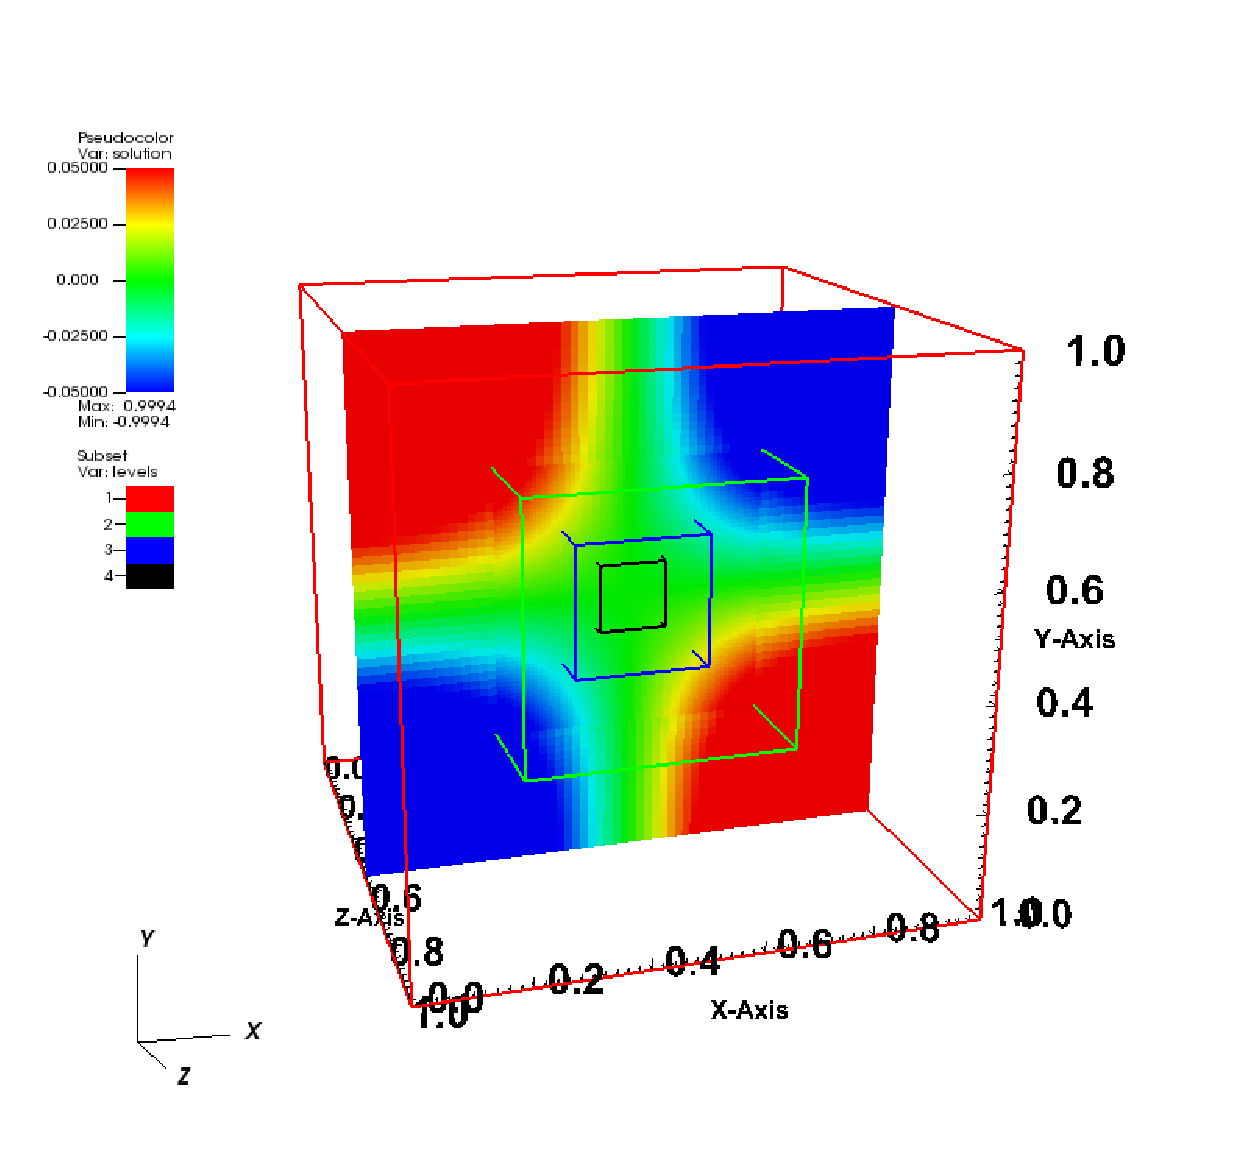
\includegraphics[scale=0.35]{NumericalSolution}
}
\subfigure[]
{
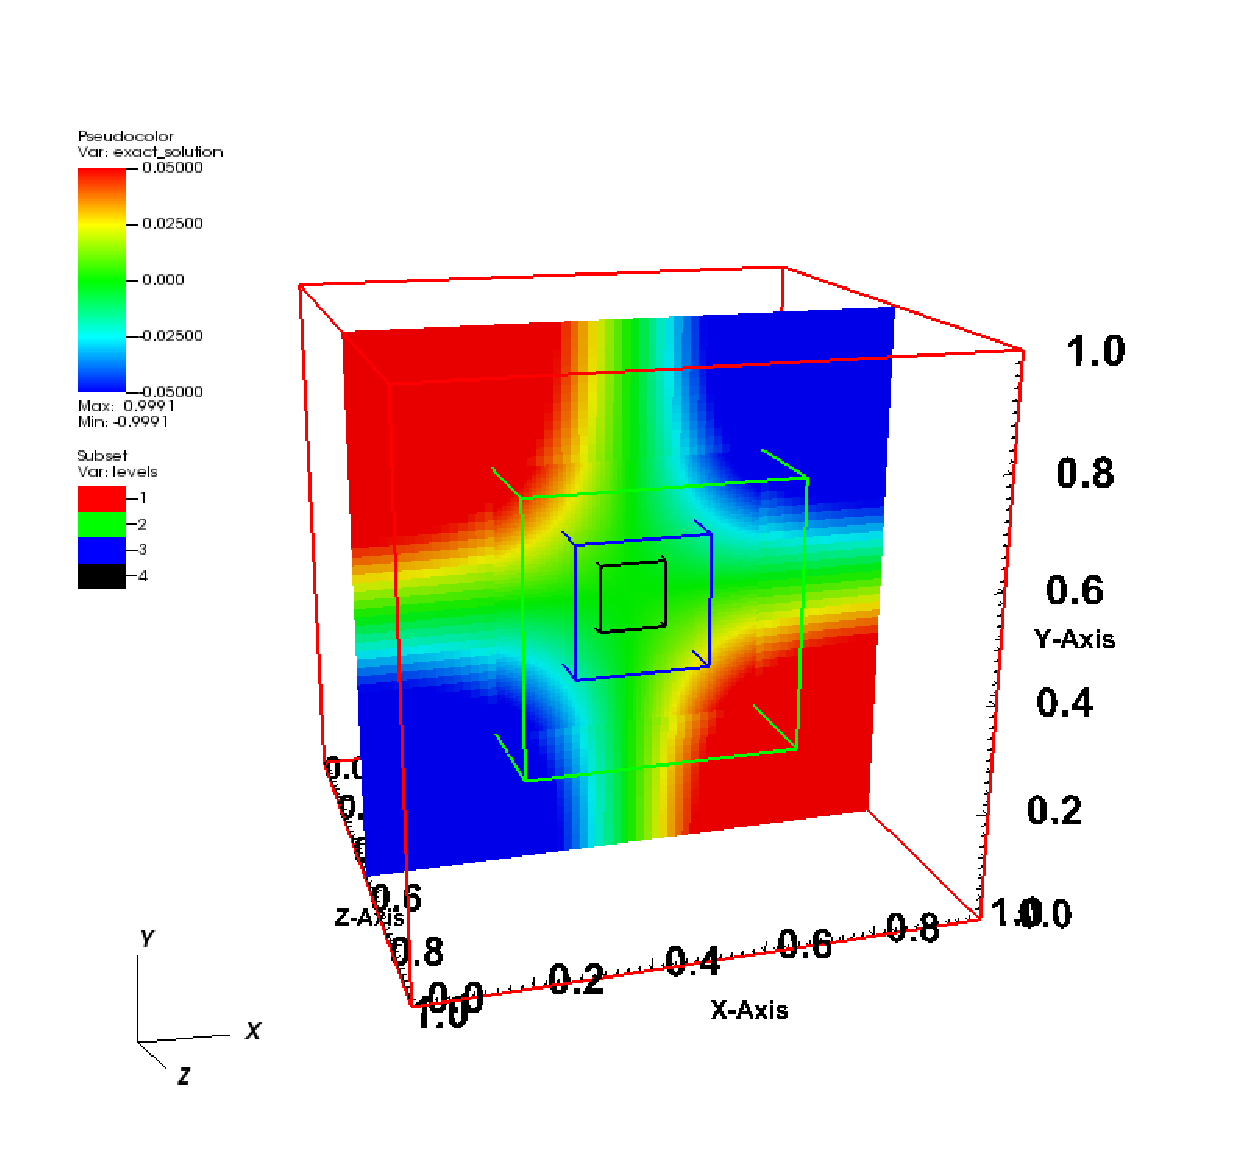
\includegraphics[scale=0.35]{ExactSolution}
}
%\subfigure[]
%{
%\includegraphics[scale=0.35]{AMRGridLevelsNumericalSlice}
%}
%\subfigure[]
%{
%\includegraphics[scale=0.35]{AMRGridLevelsExactSlice}
%}
\caption{(a) AMR grid levels and comparison of (b) numerical and (c) exact solution.} 
%and the comparison slices showing the AMR grid levels for the (d) numerical and (e) exact solutions.}
\label{fig:Comparison}
\end{figure}

\end{document}
